

\subsection{Ву}

% Нечеткие дубликаты видео — идентичные или приблизительно идентичные видео, почти
% точные копии друг друга, но отличающийся форматами файлов, параметрами кодирования,
% светоизмерительными параметрами (цветность, яркость), применением монтажа (титры, ло-
% готип, рамка), длиной и набором модификаций (вставка или удаление кадров)

\begin{frame}{Нечеткие дубликаты видео по~Ву}

    \lbgGrayBox{Копии друг друга, отличаются набором модификаций}{
        \begin{center}
        \begin{tikzcd}[column sep=5pc,ampersand replacement=\&]
            \raisebox{-.4\height}{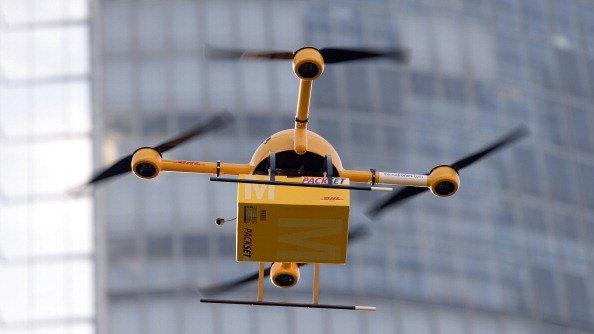
\includegraphics[height=2.5cm]{img/video/ndvex/drone/ndvex-drone-01-orig.jpg}}
                \arrow[teal, leftrightsquigarrow]{r}{\text{\color{teal}{\large $\simeq$} дубликат}}
                \arrow[teal, leftrightsquigarrow]{d}{\text{\color{teal}{\large $\simeq$} дубликат}}
                \arrow[red, leftrightarrow, dashed]{rd}{\text{\color{red}{\large $\not\simeq$} уже не~дубликат}}
            \&
            \raisebox{-.4\height}{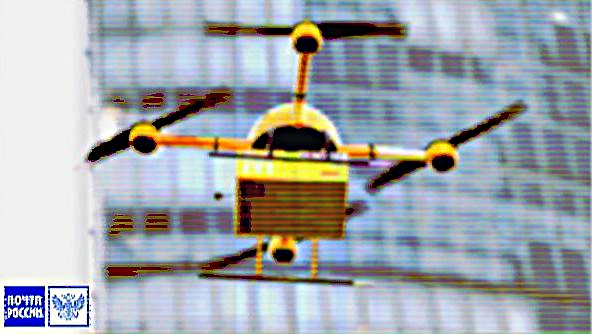
\includegraphics[height=2cm]{img/video/ndvex/drone/ndvex-drone-01-x1.jpg}}
            \\
            \raisebox{-.4\height}{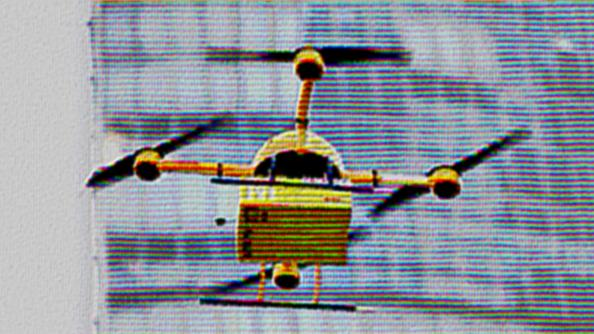
\includegraphics[height=2cm]{img/video/ndvex/drone/ndvex-drone-01-x2.jpg}}
            \&
            \raisebox{-.4\height}{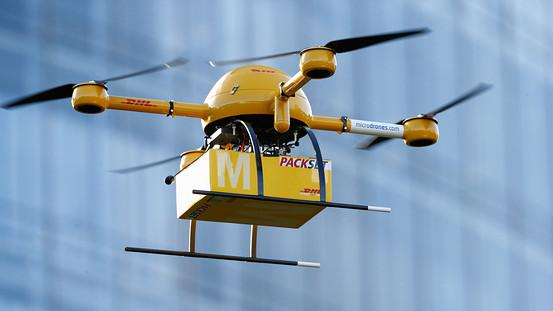
\includegraphics[height=2cm]{img/video/ndvex/drone/ndvex-drone-01-y1.jpg}}
        \end{tikzcd}
        \end{center}
    }
\end{frame}
